\chapter{Authenticating {kNN} Queries in Distributed Environment}\label{chap:knn}

In this chapter, we investigate the problem of authenticating {kNN} queries in distributed environment.

\section{Problem Formulation}\label{sec:knn:problem}

There are three parties in our system: the DO, the third-party distributed SP, and the client. The DO builds the ADS and signs the ADS to ensure the integrity of the data. The ADS and the signature are then sent to the SP\@. The distributed SP provides the service of storage and query processing. Since the SP is configured in a distributed environment, it consists of several types of nodes: $Master$, $Slave$, and $Reducer$. The $Master$ node in the SP is mainly responsible for dispatching jobs to the corresponding slaves. The $Slave$ nodes are the workers, which process the actual queries. The $Reducer$ consolidates all the partial results as well as the VOs computed by the $Slaves$ and sends them to the client. Finally, the client can verify the soundness and completeness of the results by using the VO, the DO's public key, and the root signature sent by the SP\@.

\textbf{Threat Model.}
In this system, we consider the DO as the trusted party. The SP is untrusted and can return incorrect results. Given the whole dataset $D$, the client's query point $q$, and the parameter $k$, the SP returns several results. If the result number does not match the value $k$, the client can find that some results are missing. Suppose $R_{k}=\{r_{1},r_{2},\dots,r_{k}\}$ are the $k$ true kNN results. The SP can
\begin{inlineenum}
\item return a point $p$ and $p \notin D$;
\item return a point $p \in D$ but $dist(q,p) > dist(q,r_{k})$, where $dist(\cdot,\cdot)$ denotes the Euclidean distance.
\end{inlineenum}
The first and second cases violate the soundness and completeness conditions, respectively.

The system's performance can be measured in these metrics:
\begin{inlineenum}
\item ADS construction time;
\item query processing cost;
\item client's verification time; and
\item VO size.
\end{inlineenum}
We assume that there is no data update in this system. Therefore, the ADS construction is a one-off operation by the DO and the cost can be amortized by the queries. The VO size can influence the communication overhead between the SP and the client as well as the time of client's verification. Therefore, the VO size should be minimized.

\section{Preliminaries}\label{sec:knn:prelim}

\subsection{Cryptographic Primitives}

In our solution, two cryptographic primitives are used, namely hash function and digital signature.

\textbf{Hash Function}: A one-way hash function $H(\cdot)$ transforms an arbitrary message $m$ to a fixed-length digest $H(m)$. One-way indicates that given a message $m$, the computation of $H(m)$ is easy. However, to get $m$ from $H(m)$ is computationally infeasible. In this chapter, we use SHA-1 as the hash function, which maps a given message to a 160-bit digest.

\textbf{Digital Signature}: The asymmetric signature is used to verify the integrity of the data. The DO keeps a private key and publishes the corresponding public key to the verifier. The DO signs the data using the private key and the verifier can verify the signature using the public key to ensure the integrity of the data. RSA is one of the popular asymmetric signature algorithms.

\subsection{Spatial Authenticated Data Structure}

MR-tree~\cite{10.1007/s00778-008-0113-2}, which is the combination of the R-tree and the Merkle Hash tree~\cite{10.1007/0-387-34805-0_21}, is often used to process authenticated spatial queries. Each leaf node stores the pointers pointing to the data points and the hash value of the binary concatenation of the data points. The hash value of an internal node is computed by hashing the concatenation of each child node's MBR and hash value. We give an example based on \Cref{fig:knn:local-mrtree}, which depicts the data points and their corresponding MR-tree. The leaf node $N_{3}$'s hash value is $H(a|b|c)$, where `$|$' represents the binary concatenation. The non-leaf node's hash value $H(N_{1})=H(N_{3}|H(N_{3})|N_{4}|H(N_{4}))$. Here $N_{3}, N_{4}$ represent the MBR of node $N_{3}$ and $N_{4}$, respectively. We only show three hash values in \Cref{fig:knn:local-mrtree} and other hash values are computed similarly.

\begin{figure}[t]
  \centering
  \begin{subfigure}[b]{.35\linewidth}
    \centering
    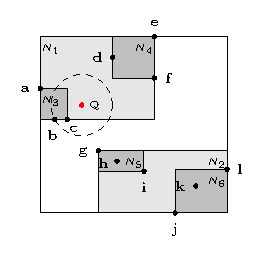
\includegraphics[width=\linewidth]{figs/knn/local-mrtree-data.pdf}
    \caption{Data}\label{fig:knn:local-mrtree:data}
  \end{subfigure}~%
  \begin{subfigure}[b]{.65\linewidth}
    \centering
    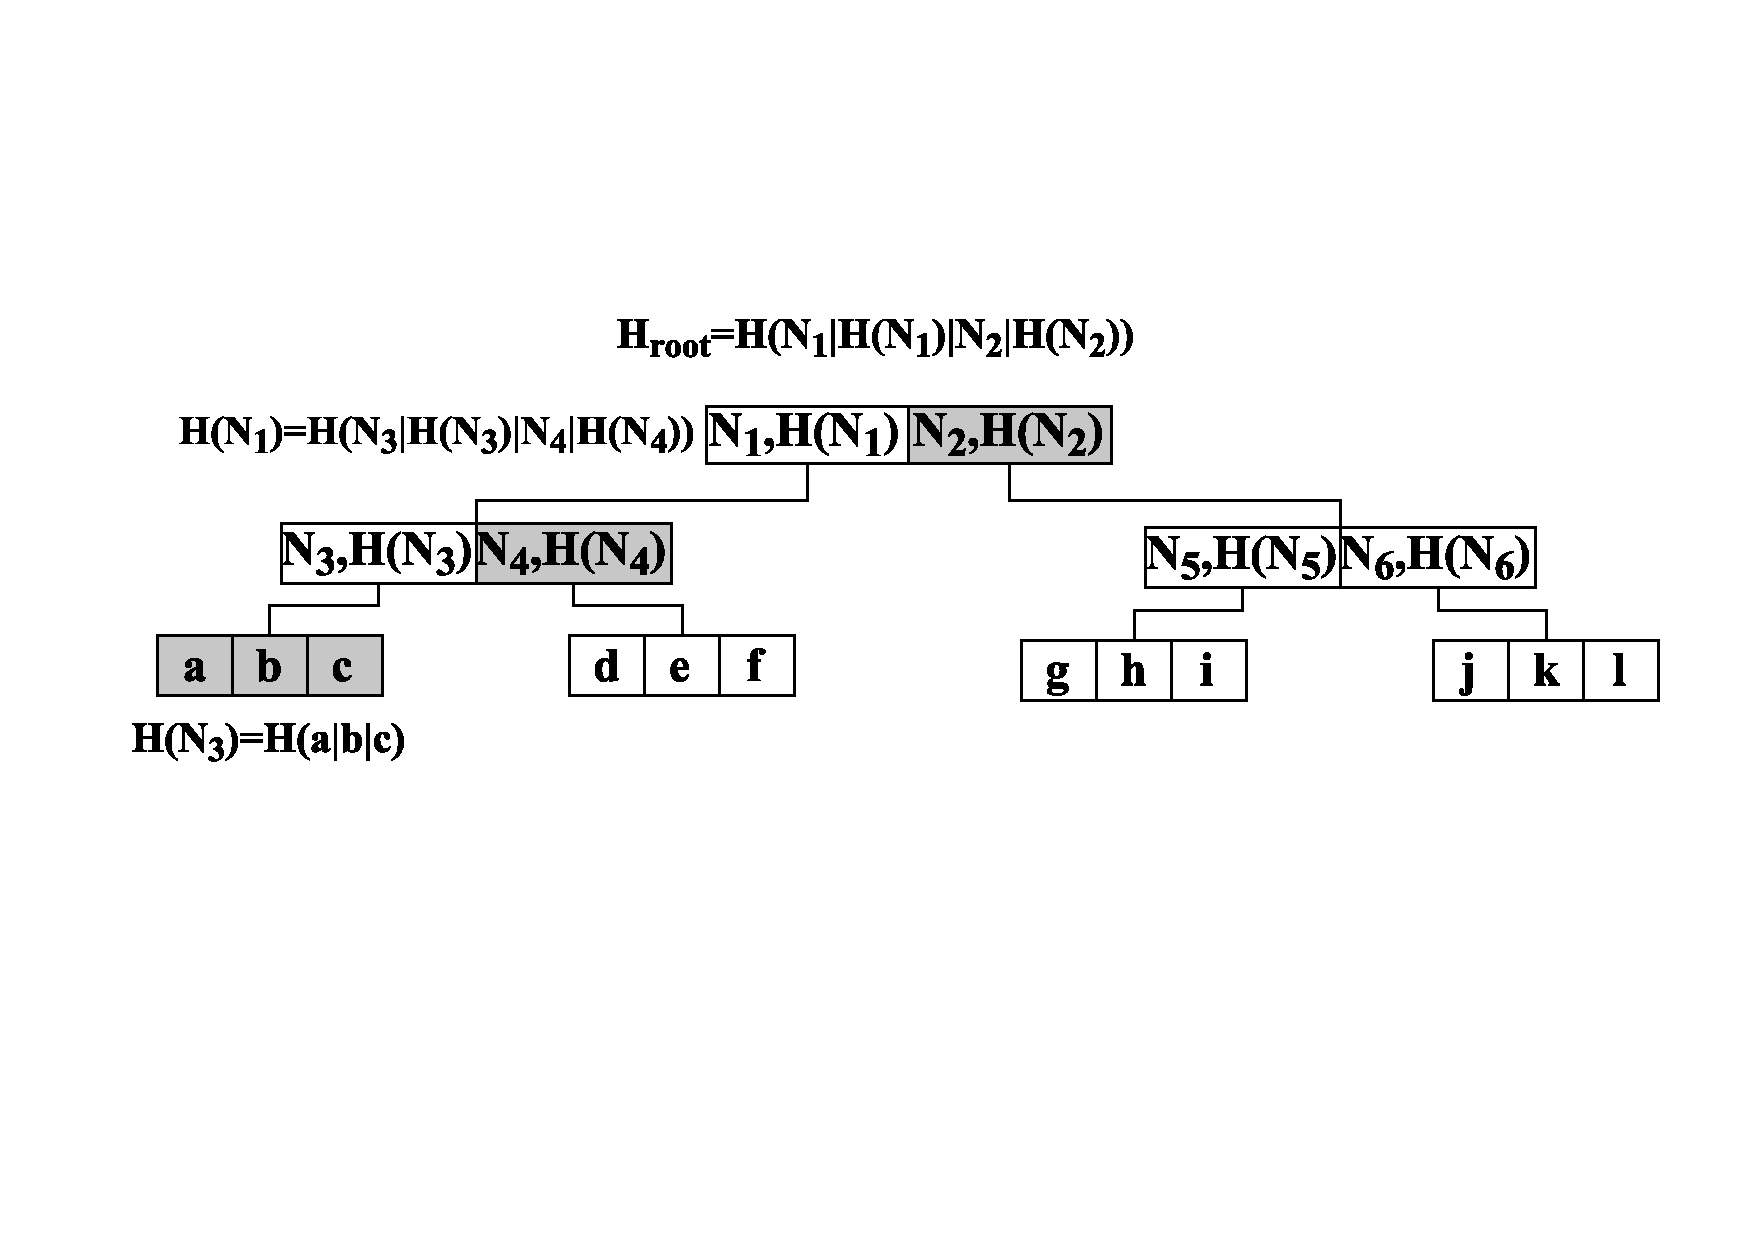
\includegraphics[width=\linewidth]{figs/knn/local-mrtree-tree.pdf}
    \caption{Index}\label{fig:knn:local-mrtree:tree}
  \end{subfigure}
  \caption{Local Authenticated {kNN} Processing}\label{fig:knn:local-mrtree}
\end{figure}

\subsection{Local Authenticated kNN Processing}
There are mainly two different methods of authenticated kNN processing based on the MR-tree. The algorithm proposed by \citeauthor{10.1007/s00778-008-0113-2}~\cite{10.1007/s00778-008-0113-2} mainly focuses on the authenticated range query and transforms the kNN query to a range query. The method separates the generation of the results and the VO\@. It first retrieves kNN results by using any kNN search method. Based on the $k$ results, we can draw a circle centered at the query point $q$ with the radius of the distance between $q$ and the $k^{th}$ result. Then, the authenticated range query is executed to generate the VO set. Another method is to generate the results and the VO set together while traversing the whole MR-tree. \citeauthor{10.1007/978-3-319-18120-2_33}~\cite{10.1007/978-3-319-18120-2_33} proposed the authentication of top-$k$ spatial keyword queries and we can transform this query to the authenticated kNN query easily. \Cref{alg:knn:knn} shows the procedure of generating the VO and results altogether.

\begin{algorithm}[t]
  \caption{Local Authenticated kNN Query}\label{alg:knn:knn}
  \KwIn{$k$, Point $q$, Root of MR-tree $\mathcal{T}_R$}
  \KwOut{Result set $RS$, Verification object $VO$}
  $RS \gets \emptyset$; $counter \gets 0$\;
  $VO \gets (\textrm{`['}, \mathcal{T}_R, \mathcal{T}_R.hash, \textrm{`]'})$\; % chktex 9
  Initialize priority queue $PQ$ and enqueue $\mathcal{T}_R$\;
  \While{$counter < k \land PQ \neq \emptyset$}{%
    $object \gets dequeue(PQ)$\;
    \eIf{$object$ is an MBR $R_i$}{%
      Enqueue each $R_{j}$ or $O_{j}$ in $R_{i}$'s child node into $PQ$\;
      Replace $R_{i}, R_{i}.hash$ with `[', each $R_{j}$, $R_{j}.hash$ (or $O_{j}$) in $R_{i}$'s child node, and `]' in $VO$\;
      }{%
      $RS \gets RS + \{object\}$\;
      $counter \gets counter + 1$\;
    }
  }
  \Return{$\langle RS, VO \rangle$}\;
\end{algorithm}

The algorithm traverses the MR-tree in a best first search manner~\cite{10.1145/320248.320255}. We maintain a priority queue $PQ$. In the while loop, the current nearest object to the point $q$ is dequeued from the priority queue $PQ$. If the object is a node rather than a data point, each of its child node $R_{j}$ will be enqueued to the $PQ$. Otherwise, the object is added to the result set because it is a point. The while loop terminates until $k$ results are collected or the $PQ$ is empty. The VO set changes along with the expansion of the object. The sign marks `[' and `]' are used to decide the scope of entries in a node and they can help the client reconstruct the root hash value. The VO set is initialized with `[', MR-tree root $\mathcal{T}_R$, $\mathcal{T}_R.hash$, and `]'. When the object is dequeued from the $PQ$, we replace $R_{i}$, $R_{i}.hash$ with `[', each $R_{j}$ and $R_{j}.hash$ (or $O_{j}$) in $R_{i}$'s child node, and `]'.

We give an example of the local authenticated kNN processing using \Cref{fig:knn:local-mrtree}. Assume that $k=2$ and the red point $Q$ is the query point. At first, the $PQ$ contains $N_{root}$ and the $VO$ is [$N_{root}, H_{root}$]. They will then be expanded to $N_1, N_2$ and [[$N_{1}$,$H(N_{1})$], [$N_{2}$,$H(N_{2})$]] respectively. Next, $N_{1}$ is removed and $N_{3}$, $N_{4}$ are added into the $PQ$. The $VO$ changes to [[[$N_{3}$, $H(N_{3})$], [$N_{4}$, $H(N_{4})$]], [$N_{2}$, $H(N_{2})$]]. Finally, points $c$ and $b$ are computed as the results and the $VO$ updates to [[[$a$,$b$,$c$], [$N_{4}$,$H(N_{4})$]], [$N_{2}$, $H(N_{2})$]]. The grey nodes in \Cref{fig:knn:local-mrtree:tree} are included in the $VO$. We omit the client verification part here as we will illustrate the verification for the distributed kNN authentication in \Cref{sec:knn:client-verification}.

\section{Distributed {kNN} Authentication}\label{sec:knn:distributed-knn}

\subsection{Distributed MR-Tree}

\begin{figure}[t]
  \centering
  \begin{subfigure}[b]{.35\linewidth}
    \centering
    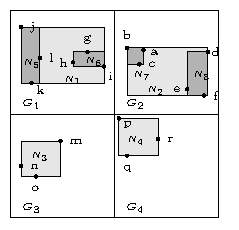
\includegraphics[width=\linewidth]{figs/knn/distributed-mrtree-data.pdf}
    \caption{Data}\label{fig:knn:distributed-mrtree:data}
  \end{subfigure}~%
  \begin{subfigure}[b]{.65\linewidth}
    \centering
    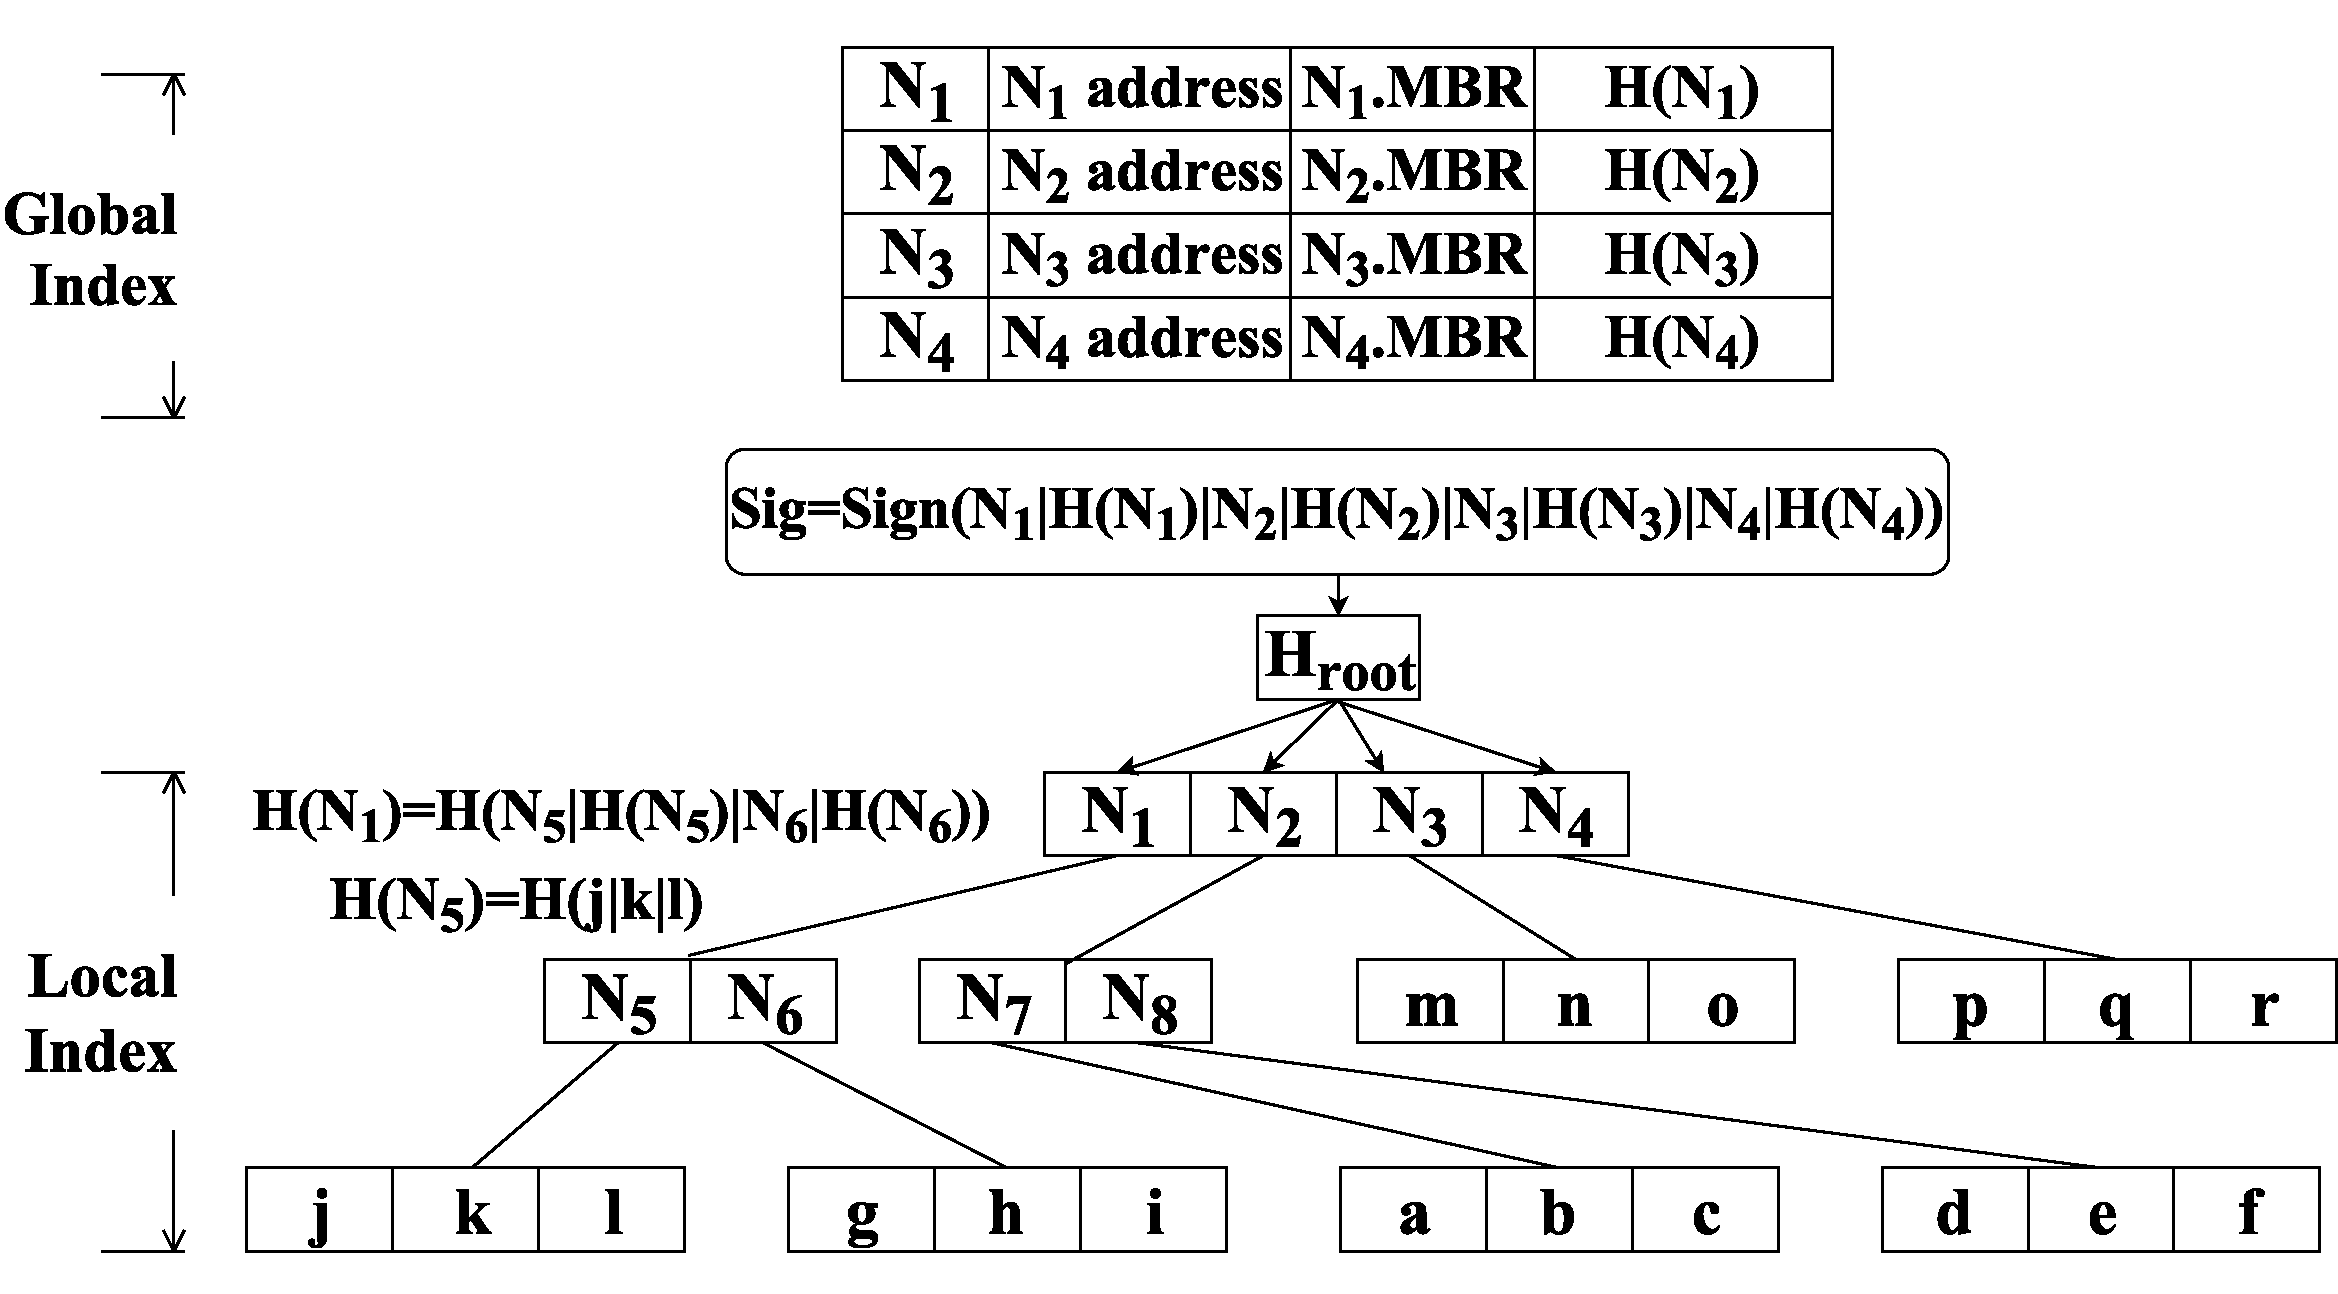
\includegraphics[width=\linewidth]{figs/knn/distributed-mrtree-tree.pdf}
    \caption{Index}\label{fig:knn:distributed-mrtree:tree}
  \end{subfigure}
  \caption{Distributed MR-tree}\label{fig:knn:distributed-mrtree}
\end{figure}

To adapt the MR-tree index structure to the distributed environment, the index structure has two layers: the local index and the global index. The DO first employs the Grid partition or the Sort-Tile-Recursive~\cite{10.1109/ICDE.1997.582015} method to partition the entire dataset into several splits. These methods guarantee that there is no overlap between any two partitions' \emph{minimum bounding rectangles} (MBRs). Thanks to this non-overlapping characteristic, only a few partitions are used to process the kNN query, which saves the computation resources. The local indexes are constructed using the data points in each partition. The global index is then constructed, and it contains each local MR-tree's root MBR and, root hash value, and the pointers towards each local index. After the construction of the index structure, the DO signs the root node of the global index using the private key. Then, the signature and the entire index will be sent to the SP\@. The $Master$ of the SP is responsible for dispatching the local indexes to the $Slaves$ according to the current workload of the distributed system. Since the global index is small, it will be stored in the main memory of all the nodes, which can speed up the kNN query processing. \Cref{fig:knn:distributed-mrtree:data} shows the four partitions using the Grid partition method. \Cref{fig:knn:distributed-mrtree:tree} depicts the entire structure of distributed MR-tree. In each partition, the data points are used to build a local MR-tree. We use $N_{1}$, $N_{2}$, $N_{3}$ and $N_{4}$ to represent the four local indexes. The global index is a directory table and can prune the search space.

\subsection{Authenticating Distributed kNN Query Processing}

For easy illustration, we first give some definitions, which will be used in the authenticating distributed kNN query processing.

\begin{definition}\label{def:knn:def1}
  Given a query point $q$ and a set of local MR-trees $T = \{T_{1}$, $T_{2}$, $\dots$, $T_{n}\}$, $T_{i}$ is a \emph{home index} if $dist(q,T_{i}.MBR) < dist(q,T_{j}.MBR)$ where $i, j\in [1 \dots n]$ and $j \neq i$. Here the $dist(\cdot,\cdot)$ denotes the minimum distance between a point and a rectangle.
\end{definition}

\begin{definition}\label{def:knn:def2}
  Given a query point $q$ and a set of current partial kNN results $\{r_{1}, r_{2}, \dots, r_{k}\}$, a \emph{rcircle} is a circle centered at $q$ with the radius of $dist(q,r_{k})$. Here the $dist(\cdot,\cdot)$ denotes the Euclidean distance.
\end{definition}

\begin{definition}\label{def:knn:def3}
  Given a \emph{rcircle} and a set of local MR-trees $T = \{T_{1}, T_{2}, \dots, T_{n}\}$, $CT$ is a set of \emph{candidate trees} if $CT \subseteq T$ and for each $CT_{i} \in CT$, $CT_{i}.MBR \cap \text{\emph{rcircle}} \neq \emptyset$ and $CT_{i} \neq \text{\emph{home index}}$.
\end{definition}

\begin{definition}\label{def:knn:def4}
  Given a set of slave nodes $Slaves = \{Slave_{1}, \dots, Slave_{n}\}$, a \emph{home slave} $HSlave \in Slaves$ is the slave which stores the \emph{home index}. And a set of \emph{candidate slaves} $CSlaves\subseteq Slaves$ are the set of slaves which stores \emph{candidate trees CT}.
\end{definition}

\begin{definition}\label{def:knn:def5}
  We define the VO computed by \emph{HSlave} is $hVO$; the VO computed by \emph{CSlaves} is $cVO$; the VO of non-processed slaves is $nVO$.
\end{definition}

\begin{definition}\label{def:knn:def6}
  We define the results computed by \emph{HSlave} are in \{$rs_{h}$\}; the results computed by \emph{CSlaves} are in \{$rs_{c}$\}.
\end{definition}

We assume that in the distributed system, queries are executed by the slaves who store the corresponding local indexes. For example, since the $HSlave$ stores the \emph{home index}, the first local kNN query should be sent to the $HSlave$ by the $Master$ and the $HSlave$ will execute the query locally.

\begin{figure}[t]
  \centering
  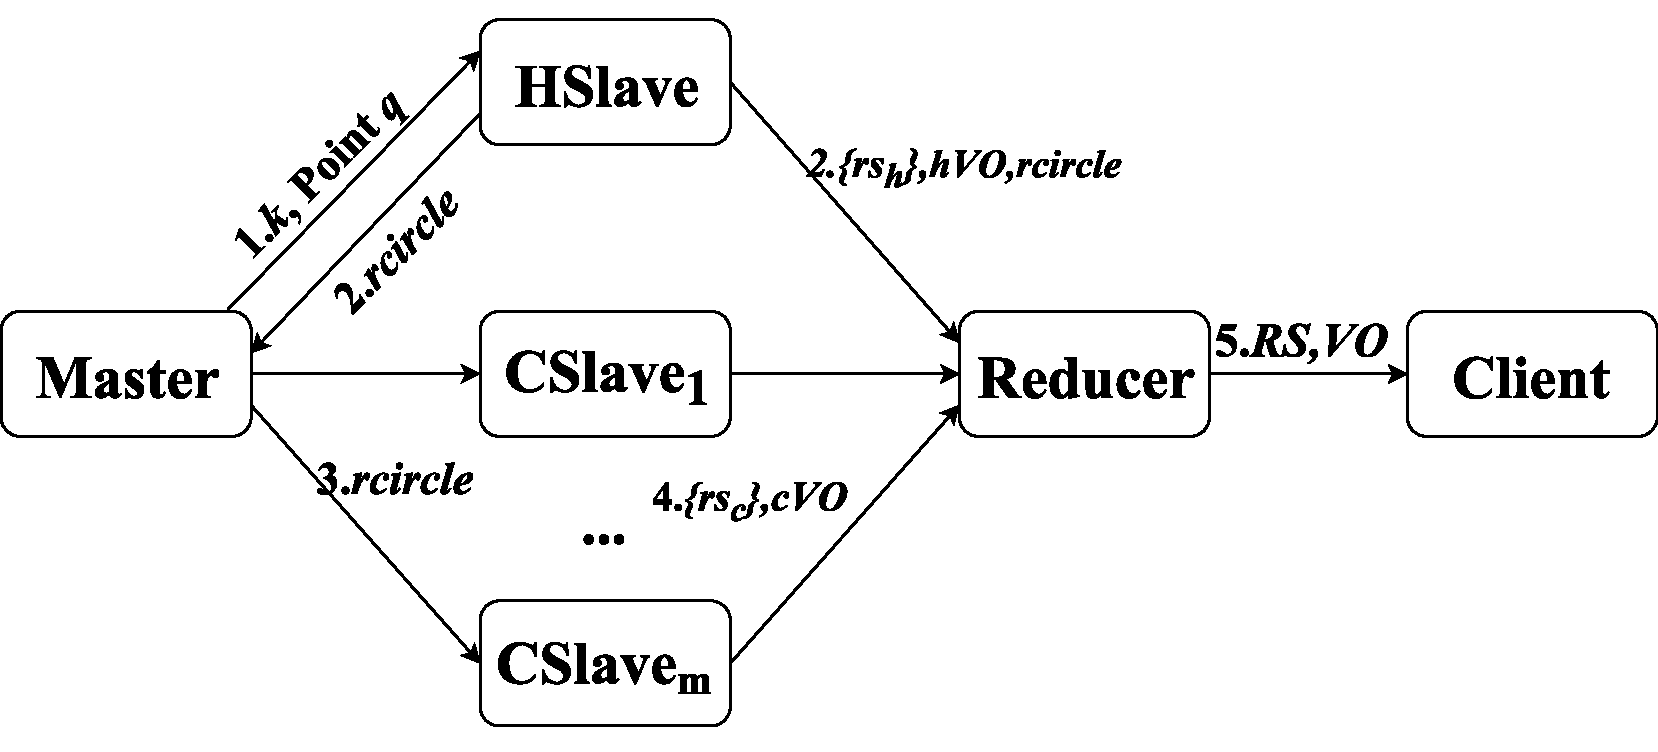
\includegraphics[width=.7\linewidth]{figs/knn/framework.pdf}
  \caption{Framework of Distributed Authenticated kNN Query}\label{fig:knn:frame}
\end{figure}

Our query authentication framework consists of three main procedures:
\begin{inlineenum}
\item the $HSlave$ processes the local authenticated kNN query to compute \{$rs_{h}$\} and $hVO$;
\item $CSlaves$ process additional range queries to compute \{$rs_{c}$\} and the $cVO$;
\item the $Reducer$ finally selects the $k$ nearest results from the partial results and generates the overall VO\@.
\end{inlineenum}
\Cref{fig:knn:frame} depicts the overview of the basic distributed kNN query processing.

The main objective is to use a small amount of partitions to compute the correct kNN results as well as the VO\@. The non-overlapping characteristic of the partition method prunes some local indexes, which saves the computation resources. The $HSlave$ first finds the local kNN results in the \emph{home index} which contains the correct results in a high probability. However, if there are some other points which are closer than the ones in $\{rs_{h}\}$, $CSlaves$ need to process extra range queries to find the correct results. The $rcircle$ is used to check whether $CSlaves$ should process the extra queries. \Cref{alg:knn:master} summarizes the procedure of the $Master$ node and the $Reducer$ node. The procedure of the $HSlave$ and the $CSlave$ is omitted because they simply compute the local queries and send the partial VO and results to the $Reducer$.

\begin{algorithm}[t]
  \caption{Distributed Authenticated kNN Procedure}\label{alg:knn:master}
  \SetKwBlock{MProc}{Master Procedure}{}
  \SetKwBlock{RProc}{Reducer Procedure}{}
  \MProc{%
    \KwIn{$k$, Point $q$}
    \KwOut{kNN request, range query requests}
    Send $kNN$ request to $HSlave$\;
    Receive $rcircle$, decide $CT$ list and $CSlaves$\;
    \If{$CT \neq \emptyset$}{
      Send \emph{range query} with $rcircle$ to the $CSlaves$\;
    }
  }
  \RProc{%
    \KwIn{$rs_{h}$, $hVO$, $rcircle$, $rs_{c}$, $cVO$}
    \KwOut{$RS$, $VO$}
    Receive $rs_{h}$, $hVO$, $rcircle$ from $HSlave$\;
    Compute $CT$ list using $rcircle$ and global index\;
    \eIf{$CT = \emptyset$}{%
      Add $hVO$ and $nVO$ to $VO$\;
      Send $rs_{h}$ and $VO$ to the $Client$\;
      }{%
      Receive \{$rs_{c}$\} and $cVO$ from $CSlaves$\;
      Add $k$ nearest results in $rs_{c}\cup rs_{h}$ to $RS$\;
      Add $hVO$, $cVO$, $nVO$ to $VO$\;
      Send $RS$ and $VO$ to the $Client$\;
    }
  }
\end{algorithm}

After receiving the kNN query from the client, the $Master$ locates the \emph{home index} and sends the kNN query request to the \emph{HSlave}. The $hVO$, $\{rs_{h}\}$ and $rcirlce$ will be computed by $HSlave$ using \Cref{alg:knn:knn} and are sent to the $Reducer$. Also, the $rcirlce$ is sent to the $Master$. Given the $rcircle$, the \emph{candidate trees} and the corresponding $CSlaves$ are identified (\Cref{def:knn:def3} and \Cref{def:knn:def4}) by the $Master$. When the $CT$ list is not empty, the $rcircle$ is sent to the $CSlaves$ by the $Master$. Each of the $CSlaves$ computes the local range query in parallel. The $Reducer$ consolidates $rs_{h}$, $\{rs_{c}\}$, $hVO$, $cVO$, and $nVO$. Then, it selects $k$ nearest results from the union of $\{rs_{h}\}$ and $\{rs_{c}\}$. The final VO list consists of $hVO$, $cVO$, and $nVO$. The $nVO$ can be derived using the global index and the $rcircle$. If a local index's MBR does not intersect with the $rcircle$, the MBR and hash value of the index will be added into $nVO$.

\begin{figure}[t]
  \centering
  \begin{subfigure}[b]{.33\linewidth}
    \centering
    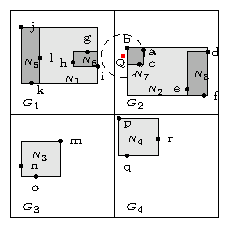
\includegraphics[width=\linewidth]{figs/knn/case1.pdf}
    \caption{Case 1}\label{fig:knn:cases:case1}
  \end{subfigure}~%
  \begin{subfigure}[b]{.33\linewidth}
    \centering
    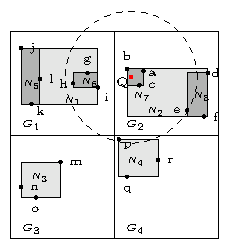
\includegraphics[width=\linewidth]{figs/knn/case2.pdf}
    \caption{Case 2}\label{fig:knn:cases:case2}
  \end{subfigure}~%
  \begin{subfigure}[b]{.313\linewidth}
    \centering
    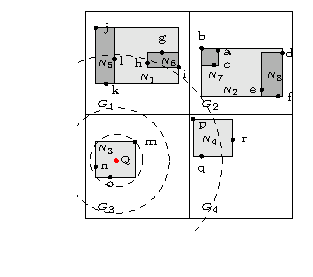
\includegraphics[width=\linewidth]{figs/knn/specialcase.pdf}
    \caption{Special Case}\label{fig:knn:cases:specialcase}
  \end{subfigure}
  \caption{Three Cases of {kNN} Processing}\label{fig:knn:cases}
\end{figure}

\Cref{fig:knn:cases} shows some cases of the distributed kNN processing. In case 1, we assume that $k$ equals $3$ and $Q$ is the query point. According to \Cref{def:knn:def1}, the \emph{home index} is $N_{2}$. Then the $Master$ sends the kNN request to the corresponding \emph{HSlave}. The $\{rs_{h}\}$ includes $\{b, c, a\}$ and the $hVO$ is $\{$[[$a, b, c$], [$N_{8}, H(N_{8})$]]$\}$. Since the $rcircle$ has no intersection with other local tree's MBR, the $CT$ list is empty. The non-processed VO set $nVO$ is \{[$N_{1}$, $H(N_{1})$], [$N_{3}$, $H(N_{3})$], [$N_{4}$, $H(N_{4})$]\}. Finally, the $Reducer$ sends the union of $hVO$ and $nVO$ and the results to the client.

In case 2, we assume that $k$ equals $4$. The query point $Q$ locates in $N_{2}$. The corresponding $HSlave$ computes the $rs_{h}=\{b, c, a, e\}$ and also the $hVO=\{$[[$a, b, c$], [$d, e, f$]]$\}$. The radius of $rcircle$ is the distance between $Q$ and point $e$. Using the global index and $rcircle$, the $Master$ node finds the $CT=\{N_{1}, N_{4}\}$ and sends the range query requests to the $CSlaves$. The two local result sets ${\{rs_{c}\}}_{N_{1}}=\{g, h, i\}$ and ${\{rs_{c}\}}_{N_{4}}=\{p\}$ are computed by each $CSlave$. Meanwhile, $cVO=\{$[[$N_{5}, H(N_{5})$], [$g, h, i$]], [$p, q, r$]$\}$ is computed. The $Reducer$ selects the $4$ nearest result points from the union of partial results and the final result set is $RS=\{b, c, a, i\}$. The local tree $N_{3}$ does not intersect with the $rcircle$, so that [$N_{3}, H(N_{3})$] will be added to the $nVO$. The final VO consists of $hVO$, $cVO$, and $nVO$.

There is a special case of the distributed kNN processing when the number of data points in a partition is less than $k$. A skewed distribution of data points may lead to this case. The previous algorithm cannot compute the correct kNN results. In this case, we double the radius of the $rcircle$ and process the range query iteratively. The $Reducer$ checks the result number and sends the message to the $Master$ if the result number is less than $k$. The $Master$ doubles the $rcircle$'s radius and the new $rcircle$ is sent to the updated $CSlaves$. This process runs iteratively until the result number exceeds $k$. \Cref{fig:knn:cases:specialcase} illustrates the special case. Assume that $k$ is $4$ and $Q$ is the query point. $N_{3}$ is the \emph{home index}. During the third iteration, we find $8$ points and the iteration terminates. Finally, the $Reducer$ selects $4$ nearest points and returns the final $RS$ and $VO$ to the client. In this special case, the VO size is rather large since the radius of $rcircle$ grows exponentially. To avoid this case, in our experiments we use the Sort-Tile-Recursive (STR)~\cite{10.1109/ICDE.1997.582015} partition method to split the dataset. The STR partition splits the near data points in the same partition and each partition has nearly the same number of data points.

\subsection{Client Verification}\label{sec:knn:client-verification}

\begin{algorithm}[t]
  \caption{Client Verification}\label{alg:knn:client-verification}
  \KwIn{$k$, Point $q$, result set $RS$, verification object $VO$}
  \KwOut{Whether the result passes the verification}
  Receive ${root}_{DO}$ and check its signature with respect to DO's public key\;
  Reconstruct MB-tree ${root}$ using $VO$\;
  \lIf{${root}_{DO} \neq {root}$}{\Return{False}}
  Extract data points and MBRs from $VO$ and put them into $rs$, $mbr$ list\;
  Sort $rs$ by distance to $q$\;
  \For{$i=[1:k]$}{%
    \lIf{$RS[i] \neq rs[i]$}{\Return{False}}
  }
  \For{$obj$~\textnormal{\textbf{in}}~$mbr$}{%
    \lIf{$dist(q,RS[k])>dist(q,obj)$}{\Return{False}}
  }
  \Return{True}\;
\end{algorithm}

The client uses the VO to verify the results' soundness and completeness. The soundness is verified first by reconstructing the root hash value of the distributed MR-tree. The root hash value is the hash value of the concatenation of each local tree's MBR and hash value. If the reconstructed hash value matches the root hash signed by the public key of the DO, the soundness is satisfied. The completeness can be verified in the following method. All of the data points and MBRs are extracted from the VO set and the client selects the first $k$ nearest data points and compares them with the $RS$. If they match, it means that no other points are closer than the RS data points. Also, all of the $MBRs$ must be farther than the $k^{th}$ result point. \Cref{alg:knn:client-verification} summarizes the procedure of client's verification.

Take \Cref{fig:knn:cases:case2} as an example. The overall VO consists of $hVO=\{$[[$a, b, c$], [$d, e, f$]]$\}$, $cVO=\{$[[$N_{5}, H(N_{5})$], [$g, h, i$]], [$p, q, r$]$\}$ and $nVO=\{$[$N_{3}, H(N_{3})$]$\}$. The client can recompute $N_{2}$ using $hVO$. $N_{7}$, $N_{8}$ as well as their corresponding hash values are derived by $\{a, b, c\}$ and $\{d, e, f\}$, respectively. $H(N_{7})$ is the hash value of the concatenation of points $a$, $b$, and $c$. Similarly, $H(N_{8})$ can be computed. $N_{2}$ and $H(N_{2})$ are generated by $N_{7}$, $N_{8}$, and their hash values. Points $g$, $h$, and $i$ are used to compute $N_{6}$ and $H(N_{6})$. $N_{1}$ with its hash value can be derived by $N_{5}$, $N_{6}$, and their hash values. $N_{4}$ and $H(N_{4})$ are computed using points $p$, $q$, and $r$ in $cVO$. The $N_{3}$ and $H(N_{3})$ are given in $nVO$. Therefore, the root hash value is computed using four local MR-trees' root hash values and MBRs. After that, the data points and MBRs are extracted from the union of VO\@. The correct results are $\{b, c, a, i\}$ and all of the non-result points will be checked whether they are closer than point $i$. Meanwhile, the MBR of $N_{5}$ and $N_{3}$ are checked whether they are farther from point $i$.

\subsection{Robustness Analysis}

\begin{lemma}\label{lem:knn:l1}
  If there is no need to invoke the range queries ($CT=\emptyset$), the local kNN result $rs_{h}$ will be the final correct results.
\end{lemma}

\begin{proof}
  This can be proved by contradiction. If there is a point $p$ which is one of the correct kNN results but not included in the local kNN result, it is either inside or outside the partition. If it is inside the partition, it should be outside the $rcircle$ since all of the points in the $rcirlce$ are added into $rs_{h}$. There are $k$ points inside the $rcircle$, so $p$ must be at least ${(k+1)}^{th}$ nearest point. This contradicts the assumption that it is one of the correct results. If it is outside the partition, as there is no intersection among the partitions, it must be farther than the current $k^{th}$ result and this contradicts the correct result assumption.
\end{proof}

\begin{lemma}\label{lem:knn:l2}
  All of the correct kNN results must reside in the $rcircle$.
\end{lemma}

\begin{proof}
  This can be proved by contradiction. Suppose there is a correct kNN result $p$ which resides outside the $rcircle$. The radius of $rcircle$ is computed by the distance between the $k^{th}$ current nearest point and the query point. There are at least $k$ data points inside the $rcircle$ because apart from the $k$ local results, there are probably some points in other partitions that are closer than the current $k^{th}$ point. Since $p$ is outside the $rcircle$, it is at least the ${(k+1)}^{th}$ nearest point, which contradicts the assumption.
\end{proof}

\begin{theorem}
  \Cref{alg:knn:master} can produce the correct result set.
\end{theorem}

\begin{proof}
  This can be proved using \Cref{lem:knn:l1} and \Cref{lem:knn:l2}.
\end{proof}

\Cref{alg:knn:client-verification} summarizes the procedure of client verification. The root hash reconstruction guarantees the \emph{soundness} of the results and the distance comparison protects the \emph{completeness}. We now give the following theorem of its correctness of verification.

\begin{theorem}\label{thm:knn:verify}
  \Cref{alg:knn:client-verification} verifies the soundness and completeness of the results and can detect the threats mentioned in \Cref{sec:knn:problem}.
\end{theorem}

\begin{proof}
  If the adversary returns a fictitious point, which is not included in the dataset, the reconstructed root hash must be different from the signed hash value received from the DO because of the collision-resistance characteristic of the hash function. If one data point changes, its corresponding hash value will be different, resulting in the change of the root hash value of MR-tree. Without knowing the secret key, the SP cannot generate a valid signature of the wrong root hash value, which means that the signature is unforgeable. Therefore, the violation of soundness can be detected. If the reconstructed hash value matches the signed one, the incorrect result point must reside in the VO set but farther than the correct results. After the client sorts all the data points in the VO set by distance and gets the first $k$ nearest points, the client can notice the difference between $k$ points extracted from the VO and the points in RS\@. Then the results cannot pass the verification of the completeness.
\end{proof}

\section{Optimization of VO size}\label{sec:knn:opt}

The VO size determines the communication cost and also the client verification time. In this section, we focus on the optimization of the VO size. Intuitively, the $rcircle$ decides the VO size. A larger $rcircle$ makes more nodes to be visited and hence and more data points to be added to the VO\@. Therefore, the objective is to reduce the radius of the $rcircle$. As we can see in \Cref{fig:knn:cases:case2}, the $rcircle$ is much bigger than the circle with the radius of the distance between $Q$ and point $i$. This is because the distance between $Q$ and $e$ is larger than the distance between $Q$ and $i$. In \Cref{alg:knn:master}, the $rcircle$ is decided by the local results in \emph{home index} and will not change during the whole procedure. To compute the minimum $rcircle$, the optimized algorithm adds the sequential computation of the $rcircle$ before the parallel authenticated range query in \Cref{alg:knn:master}.

\begin{algorithm}[t]
  \caption{VO Optimization Algorithm}\label{alg:knn:opt}
  \SetKwBlock{MProc}{Master Procedure}{}
  \MProc{%
    \KwIn{$k$, Point $q$}
    \KwOut{kNN request, range query requests}
    Send $kNN$ request to $HSlave$\;
    Receive $rcircle$\;
    Compute $CT$ list and decide $CSlaves$\;
    \If{$CT \neq \emptyset$}{%
      Sort $CT$ list with minimum distance\;
      \For{$i = [1:|CT|]$}{%
        \lIf{$rcircle$ not intersects $CT[i].MBR$}{\textbf{break}}
        Send $rcircle$ to $CSlave[i]$\;
        Receive $rs_{c}$\;
        $rs_{h} \gets rs_{h} + rs_{c}$\;
        Select $k^{th}$ nearest point $obj$ in $rs_{h}$\;
        Update $rcircle$'s radius with $dist(obj, q)$\;
      }
      Recompute $CSlaves$ using final $rcircle_{f}$\;
      Send $rcircle_{f}$ to $HSlave$ and $CSlaves$\;
    }
  }
\end{algorithm}
